\documentclass[189]{pset}

% ================================================================== %
%                                                                    %
%                              Document                              %
%                                                                    %
% ================================================================== %

% ----------------------- Header formatting ------------------------ %

\name{Forest Kobayashi}
\class{Math of Big Data}
\season{Summer}
\prof{Gu}
\assignment{6}
\duedate{05/22/2018}
\dueday{Tuesday}
\problems{1, 2}
\acknowledgements{{}, {}}
\onTime{0}

\comments{\textbf{Comments:} Feel free to work with other students,
  but make sure you write up the homework and code on your own (no
  copying homework \textit{or} code; no pair programming). Feel free
  to ask students or instructors for help debugging code or whatever
  else, though.

  The starter files for problem 2 can be found under the Resource tab
  on course website. The plot for problem 2 generated by the sample
  solution has been included in the starter files for reference.
  Please print out all the graphs generated by your own code and
  submit them together with the written part, and make sure you upload
  the code to your Github repository.}

\lfoot{Due Wednesday, May 23rd 2018}

\begin{document}

% --------------------------- Problem 1 ---------------------------- %

  \section{(Murphy 11.3)}
  \textbf{EM for Mixtures of Bernoullis:}
  Show that the M step for ML estimation of a mixture of Bernoullis is
  given by
  \[
    \mu_{kj} = \frac{\sum_i r_{ik}x_{ij}}{\sum_i r_{ik}}.
  \]
  Show that the M step for MAP estimation of a mixture of Bernoullis
  with a $\beta(a,b)$ prior is given by
  \[
    \mu_{kj} = \frac{\pn{\sum_i r_{ik}x_{ij}} + a - 1}{\pn{\sum_i
        r_{ik}} + a + b - 2}.
  \]
  \hrulefill

  \section*{Solution:}
  \begin{enumerate}
  \item In 5.4.2.1, we have that for $X \sim \mrm{Ber}(\theta)$, the
    log likelihood for a single sample is
    \[
      \log\pn{p\pn{X \MID \theta}} = X \log\pn{\theta} + (1-X)
      \log\pn{1 - \theta}.
    \]
    hence, for a mixture of bernoullis, we have
    \begin{align*}
      \ell\pn{\bm{\mu}}
      &= \sum_i \sum_k r_{ik} \log \pn{ \PP (\vx_i \mid
        \bm{\theta}_k)} \\
      &= \sum_i \sum_k r_{ik} \sum_j \vx_{ij} \log\pn{\bm{\mu}_{kj}} +
        (1-\vx_{ij}) \log\pn{1 - \bm{\mu}_{kj}}
    \end{align*}
    differentiating, the $k,j$ sums go away (since we're looking at a
    particular $\mu_{kj}$), and we have
    \begin{align*}
      0 &=
      \od{\ell\pn{\bm{\mu}}}{\bm{\mu}_{kj}}\\
      &= \sum_i r_{ik} \pn{\frac{\vx_{ij}}{\mu_{kj}} - \frac{1 -
        \vx_{ij}}{1 - \mu_{kj}}} \\
      \sum_i r_{ik} \frac{\vx_{ij}}{\mu_{kj}} + \frac{\vx_{ij}}{1 -
      \mu_{kj}}
      &= \sum_i r_{ik} \frac{1}{1 - \mu_{kj}} \\
      \sum_i r_{ik} \vx_{ij} \pn{\frac{1 - \mu_{kj}}{\mu_{kj}} + 1}
      &= \sum_i r_{ik} \\
      \sum_i r_{ik}\vx_{ij} \pn{\frac{1}{\mu_{kj}}}
      &= \sum_i r_{ik} \\
      \mu_{kj}
      &= \frac{\sum_i r_{ik} \vx_{ij}}{\sum_i r_{ik}}
    \end{align*}
  \item Adding in a beta prior, we have
    \begin{align*}
      \ell\pn{\bm{\mu}}
      &= \sum_i \sum_k \bk{r_{ik}\log\pn{\PP\pn{\vx_i \MID
        \bm{\theta}_k}}} + \log\pn{\bm{\mu}_k} \\
      &= \sum_i \sum_k r_{ik} \sum_j \bk{\vx_{ij}
        \log\pn{\bm{\mu}_{kj}} + (1-\vx_{ij}) \log\pn{1 -
        \bm{\mu}_{kj}}} + (a-1) \log \pn{\bm{\mu}_{kj}} + (b-1) \log
        \pn{1-\bm{\mu}_{kj}}
    \end{align*}
    hence
    \begin{align*}
      0
      &= \od{\ell\pn{\bm{\mu}}}{\bm{\mu}_{kj}} \\
      &= \sum_i \pn{r_{ik} \bk{\frac{\vx_{ij}}{\mu_{kj}}} - \frac{1 -
        \vx_{ij}}{1 - \mu_{kj}}} + \frac{a-1}{\mu_{kj}} -
        \frac{b-1}{1 -\mu_{kj}}\\
      &= \frac{\sum_i (r_{ik} \vx_{ij}) + a - 1}{\mu_{kj}} -
        \frac{\sum_i (r_{ik} (1 - \vx_{ij})) + b - 1}{1 - \mu_{kj}} \\
      &= \frac{1}{\mu_{kj} (1-\mu_{kj})} \pn{\sum_i \pn{r_{ik}
        \vx_{ij}} + a - 1}\pn{1 - \mu_{kj}} - \pn{\sum_i
        (r_{ik}(1-\vx_{ij})) + b - 1}\mu_{kj}
        \shortintertext{to avoid clutter, let $C_0 = \sum_i r_{ik}
        \vx_{ij}$, and $C_1 = \sum_i r_{ik}$}
      &= \frac{1}{\mu_{kj} (1-\mu_{kj})} \bk[Big]{\pn{C_0 + a -
        1}\pn{1 - \mu_{kj}} + \pn{C_0 - C_1 - b + 1}\mu_{kj}} \\
      &= \frac{1}{\mu_{kj} (1-\mu_{kj})} \bk[Big]{C_0 + a - 1 -
        \cancel{C_0 \mu_{kj}} - a\mu_{kj} + \mu_{kj} +
        \cancel{C_0 \mu_{kj}} - C_1\mu_{kj} - b\mu_{kj} + \mu_{kj}}  \\
      &= \frac{1}{\mu_{kj}(1-\mu_{kj})} \bk[Big]{C_0 + a - 1 - a
        \mu_{kj} - C_1 \mu_{kj} - b\mu_{kj} + 2 \mu_{kj}}\\
      (C_1 + a + b - 2)\mu_{kj}
      &= C_0 + a - 1 \\
      \mu_{kj}
      &= \frac{C_0 + a - 1}{C_1 + a + b - 2}
    \end{align*}
    as desired. \qed
  \end{enumerate}
  \clearpage

% --------------------------- Problem 2 ---------------------------- %

  \section{(Lasso Feature Selection)}
    In this problem, we will use the online news popularity dataset we
    used in hw2pr3. In the starter code, we have already parsed the
    data for you. However, you might need internet connection to
    access the data and therefore successfully run the starter code.

    First, ignoring undifferentiability at $x=0$, take $\frac{\partial
      |x|}{\partial x} = \mathrm{sign} (x)$. Using this, show that
    $\nabla \|\vx\|_1 = \mathrm{sign}(\vx)$ where $\mathrm{sign}$ is
    applied elementwise. Derive the gradient of the $\ell_1$
    regularized linear regression objective
    \begin{align*}
      \text{minimize: } & \|A\vx - \vb\|_2^2 + \lambda \|\vx\|_1
    \end{align*}

    Then, implement a gradient descent based solution of the above
    optimization problem for this data. Produce the convergence plot
    (objective vs. iterations) for a non-trivial value of $\lambda$.
    In the same figure (and different axes) produce a `regularization
    path' plot. Detailed more in section 13.3.4 of Murphy, a
    regularization path is a plot of the optimal weight on the $y$
    axis at a given regularization strength $\lambda$ on the $x$ axis.
    Armed with this plot, provide an ordered list of the top five
    features in predicting the log-shares of a news article from this
    dataset (with justification).

  \hrulefill

  \section*{Solution:}
    We have
    \begin{align*}
      \nabla \norm{\vx}_1
      &= \nabla \sum_{i} \abs{x_i} \\
      &= \mrm{sign} (\vx)
    \end{align*}
    hence, with respect to $\vx$
    \begin{align*}
      \nabla \pn{\norm{A\vx - \vb}_2^2 + \lambda \norm{\vx}_1}
      &= \nabla \pn{\vx^\T A^\T A \vx - 2\vb^\T A \vx + \vb^\T \vb} +
        \lambda \ \mrm{sign}(\vx) \\
      &= 2 A^\T A \vx - 2\vb^\T A + \lambda\ \mrm{sign}(\vx)
    \end{align*}
    After fixing a pernicious off-by-one error, we see that the most
    important features are
    \begin{enumerate}[label=\arabic*.]
      \item \texttt{timedelta}
      \item \texttt{weekday\_is\_wednesday}
      \item \texttt{weekday\_is\_thursday}
      \item \texttt{weekday\_is\_friday}
      \item \texttt{weekday\_is\_saturday}
    \end{enumerate}
    which we can see in the lasso plot below, because they have the
    largest coefficients associated with them.
    \begin{figure}[H]
      \centering
      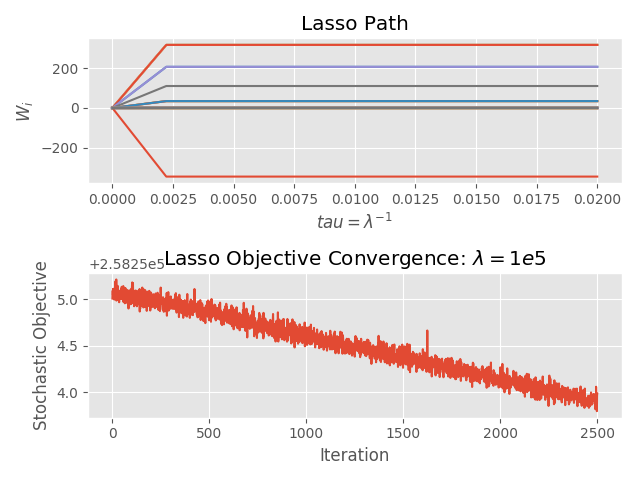
\includegraphics{hw7pr2_lasso.png}
      \caption{plot}
      \label{fig:w}
    \end{figure}
\end{document}
